\documentclass{template}

\usepackage{graphicx,parskip,appendix,float,geometry}
%  http://tex.stackexchange.com/questions/13509/biblatex-in-a-nutshell-for-beginners
%  http://tex.stackexchange.com/questions/108605/getting-a-harvard-style-list-of-references-using-biblatex
\graphicspath{ {C:\Users\Jack\Desktop\bcuThesisTemplate-master (1)\ThesisTemplate} } 
\usepackage{DejaVuSans}
\usepackage{pdfpages}
\geometry{
 a4paper,
 total={150mm,240mm},
 left=35mm,
 top=25mm,
 }
% BCU Harvard Referencing
%  http://library.bcu.ac.uk/references.pdf

% Citing   use \autocite, \parencite, or \textcite rather than \cite.
%  http://tex.stackexchange.com/questions/102662/harvard-reference-using-biblatex
%  https://www.sharelatex.com/blog/2013/07/31/getting-started-with-biblatex.html
%  http://guides.library.yale.edu/bibtex/home
%\usepackage[backend=bibtex, style=authoryear, firstinits=true, ]{biblatex}
%\addbibresource{thesis.bib}

%  Fontsizes  
%  https://en.wikibooks.org/wiki/LaTeX/Fonts

%\AtBeginBibliography{\footnotesize}
% \DeclareFieldFormat => Remove Quotes from article Titles
%  http://tex.stackexchange.com/questions/94089/remove-quotes-from-inbook-reference-title-with-biblatex
%\DeclareFieldFormat[inbook,inproceedings,article,phdthesis,mastersthesis]{citetitle}{#1}
%\DeclareFieldFormat[inbook,inproceedings,article,phdthesis,mastersthesis]{title}{#1}

\usepackage{natbib}
\newcommand*{\urlprefix}{Available from: }
\newcommand*{\urldateprefix}{Accessed }
\bibliographystyle{bath}
\usepackage{tocloft}
\newcommand{\listequationsname}{List of Equations}
\newlistof{myequations}{equ}{\listequationsname}
\newcommand{\myequations}[1]{%
\addcontentsline{equ}{myequations}{\protect\numberline{\theequation}#1}\par}
\setlength{\cftmyequationsnumwidth}{2.5em}% Width of equation number in List of Equations
%  Documentation
%  http://mirror.switch.ch/ftp/mirror/tex/macros/latex/contrib/biblatex/doc/biblatex.pdf
\renewcommand*\familydefault{\sfdefault}
\usepackage[T1]{fontenc}
%  http://tex.stackexchange.com/questions/86120/font-size-of-figure-caption-header
\usepackage[font=small]{caption}
\usepackage[ruled] {algorithm2e}
\usepackage{url,amsmath,amssymb,fancybox,listings,pdfpages,caption,multicol,datetime,rotating, booktabs}
%\usepackage[usenames,dvipsnames]{color}
\usepackage[pagebackref=false,pdffitwindow=true]{hyperref}
%NOTE: The hyperref usepackage should be the last \usepackage!!
%NOTE: When pagebackref=true an error will appear at the end of compiling. press `q' to ignore
%NOTE: Referencing Algorithms does not work if this usepackage is before the hyperref include.!!
%NOTE: This is a comment, ignored when the document is compiled
%NOTE: The following document configuration settings generally do not need to be modified
%NOTE: More packages may need to be added to provide additional functionality

%  http://tex.stackexchange.com/questions/7546/how-to-get-latex-symbol-in-document
\newcommand{\latex}{\LaTeX\ }
\newcommand{\authorName}{Jack Wolverson}
\newcommand{\reportTitle}{Training an artificial intelligence usingvarious machine learning techniques topredict the outcome of a sporting event:Could a model be trained to effectivelypredict this outcome?}
\newcommand{\degreeAward}{BSc in Computer Science } 

\hypersetup{
    pdftitle    = {\reportTitle},
    pdfauthor   = {\authorName},
    pdfsubject  = {Computer Science},
    pdfkeywords = {Comma separated list of keywords},
    colorlinks  = true, anchorcolor = blue, filecolor = blue, urlcolor = blue,
    linkcolor   = blue,    %NOTE: change (blue) to (colIdentifier) to have links within the document in Black
    citecolor   = blue,    %NOTE: change (blue) to (colIdentifier) to have citation links within the document in Black
}

\definecolor{colBackGrnd}{rgb}{1,1,0.8}
\definecolor{colKeys}{rgb}{0,0,1}
\definecolor{colIdentifier}{rgb}{0,0,0}
\definecolor{colComments}{rgb}{0,.5,0}
\definecolor{colString}{rgb}{0,0,1}
\definecolor{colWhite}{rgb}{1,1,1}

\newcommand{\MyHookSign}{\hbox{\ensuremath\hookleftarrow}}

\newtheorem{Theorem}{Theorem}
\newtheorem{Proposition}[Theorem]{Proposition}
\newtheorem{Lemma}[Theorem]{Lemma}
\newtheorem{Proof}[Theorem]{Proof}
\newtheorem{Remark}[Theorem]{Remark}
\newtheorem{Claim}[Theorem]{Claim}
\newtheorem{Example}[Theorem]{Example}
\newtheorem{Definition}[Theorem]{Definition}

%NOTE: Setup for including program listings
\lstset{%
    float=H,
    basicstyle=\ttfamily\footnotesize,
    identifierstyle=\color{colIdentifier},
    keywordstyle=\color{colIdentifier}, %
    stringstyle=\color{colIdentifier},
    commentstyle=\color{colIdentifier}, %
    columns=flexible,
    tabsize=2,
    frame=single,
    extendedchars=true, %
    showspaces=false,
    showstringspaces=false,
    numbers=left, %
    numberstyle=\footnotesize,
    breaklines=true,
    prebreak={\space\MyHookSign},
    language=Java,
    backgroundcolor=\color{colBackGrnd},
    breakautoindent=true, %
    captionpos=b%
}

\sloppy %NOTE: To ensure the Right Hand Margin is used (Especially for long URLS)
%NOTE: END of the document configuration settings
\begin{document}
\DeclareGraphicsExtensions{.png,.gif,.pdf}
%NOTE: When inserting Figures if the extension of the graphic file is not provided LaTeX will automatically search
% for the extensions declared above, in the order declared.

\title{\huge{Training an artificial intelligence using various machine learning techniques to predict the outcome of a sporting event: Could a model be trained to effectively predict this outcome?}}
\author{Jack Wolverson}
\degreetitle{\degreeAward} % Replace with appropriate degree
\rpttype{BSc}    % Replace PhD / MSc  / BSc.
\principaladviser{Emmett Cooper}

\beforeabstract
\prefacesection{Abstract}
Neural Networks use in sports prediction has gone on for many years. This research project will investigate how various machine learning techniques could be utilised to create predictive models for the outcome of sporting events, with a particular focus on racing. The model/s produced will then be tested and evaluated to measure the effectiveness and measure how successful the models are at the task determined. The conclusion of this report will draw upon the research an give a final few words on the projects research and the research artefact, as well as, looking at any further research that could take place.
\prefacesection{Acknowledgements}
I would like to thank my friends and family for offering their support throughout the year and during the process of this project. Additionally, I would like to thank my supervisor for supporting and guiding this project.
\afterpreface \afterabstract

\listofmyequations

\chapter{Introduction}
\pagenumbering{arabic} \setcounter{page}{1}

\section{Background}

With the evolution of machine learning and predictive modelling being used to forecast the outcome of sporting events, as well as analysing every moment of a particular game to improve team performance, find an opponent's weakness and improve tactics, could an artificial intelligence be trained to predict the outcome of a given race with reasonable accuracy? Predictive modelling techniques have previously been used in forecasting the outcome of sporting \cite{2015arXiv151105837K,trap2493,5647440}.
This project will research the various techniques used by several parties such as the teams themselves, bookmakers and spectators to see they can be used to predict the outcome of certain events. The research into how certain parties predict the outcome of the event is not the only research that will take place, research into data collection will be done, as well as the main body of the research which is to find a suitable set of algorithms to train the model on.

\section{Aim}
To investigate how various machine learning techniques could be utilised to create predictive models for the outcome of sporting events, with a particular focus on racing.


\section{Objectives}

\begin{enumerate}
    \item To review various techniques previously used to predict the outcome of sporting events and, more specifically, the results of races.
    \item To review appropriate evaluation techniques which can be used to assess the performance of the predictive techniques identified.
    \item To identify an appropriate method of data collection for creating a dataset which can be leveraged by the system for the purpose of training and testing.
    \item Implement a system which utilises appropriate machine learning techniques identified during the background research stage to build models for predicting the outcome of a given sporting event (e.g. a horse race).
    \item Evaluate the capabilities of the model via the techniques previously identified.
\end{enumerate}

\section{Product}
The main product at the end of this project will be the research seeing if a model can be trained to correctly predict the outcome of a race. A product will be developed, this research artefact is the model itself that the research led to being built, and also helped further the research into this topic. In this section, the product will be referred to as the research artefact. This is due to the research being the main focus of this project and not a final product. The main part of the research will be the choices of which algorithms will be used to train the model, to further the research into this topic.
The artefact will be the model that trains off of data collected on a set of races, after the model is trained it will be tested on another part of the data. This test data will be used to determine the accuracy of the model.
\section{Rationale}
Artificial intelligence and machine learning are having an impact on the way sports are analysed \cite{MIN2008551} . Specific groups are going to benefit from the research that is to take place in many different ways. Some of these ways are: Bookmakers may benefit from such research into racing due to there being a way that a horse can pay out more for placing than it can by winning \cite{levitt_2014}. If a horse is to pay out more for placing than winning, than bookmakers could leverage a system to tell them the possibility of both outcomes and adjust odds so they don't have to pay out as much. Another benefit of research surrounding not just racing but sports as a whole is having real time analytics fed into a decision-making system for coaches to the be given processed data to make decisions off of \cite{7029116}. Finally, another party benefiting from such a system that will be built are spectators of the sport, spectators could benefit in many ways, one of which is that they can know whether or not to place a bet on how likely the outcome is to happen.
\\ \\

\section{Chapter List}

A short summary of the chapters of this report.
\begin{itemize}
	\item \textbf{Chapter \ref{ch:Literature Review}} Literature Review. This chapter looks at previous works surrounding relevant topics to this project.
	\item \textbf{Chapter \ref{ch:Background Research}} Background Research. Research into topics concluded upon in the literature review.
	\item \textbf{Chapter \ref{ch:Design}} Design. Looking into the design on the artefact.
	\item \textbf{Chapter \ref{ch:Data}} Dataset. A summary upon the dataset used in this project. 
	\item \textbf{Chapter \ref{ch:Implementation}} Implementation of the artfact is discussed in this chapter.
	\item \textbf{Chapter \ref{ch:Evaluation}} Evaluation \& Testing. This chapter deals with the evaluation and testing of the artefact.
	\item \textbf{Chapter \ref{ch:Conclusion}} Conclusion. The conclusions of the report are presented.
\end{itemize}


\chapter{Literature Review}\label{ch:Literature Review}

This section will look into and review previous works surrounding core aspects of this project. These topics are; the algorithm used in similar systems to help decide the algorithm that will be leveraged to train the machine learning model that is the research artefact. The data collection techniques such as data scraping that could be used to build the data set needed to train and test the model. Finally, the third topic is the evaluation metrics that could be used as a tool to help evaluate the model once it has been built.


A plethora of papers were found for this review. These have been narrowed down to the most relevant for each topic.These had to be reviewed and narrowed down to those containing the most appropriate content.During researching many papers were found that were slightly outside the scope of the topics. these papers had relevant information but concentrated on topics hat were not needed for this review.Finally, the papers selected where either a journal, journal articles or conference proceedings


\section{Algorithm Comparison}
The most common algorithm used in the context of horse racing prediction is a type of neural network. \cite{Davoodi2010HorseRP} states that neural networks are the appropriate method for this context. Two of the three papers to be compared in this section both provide a comparison of four or five different neural network algorithms and discus the benefits of using certain ones over others. The third paper for this section uses fuzzy logic and discuss the benefits of using fuzzy logic over neural networks. These will be compared in depth below. 

\cite{HRFL}explores the use of Fuzzy Logic  to build an artificial intelligence to predict the outcome of a horse race. \cite{HRFL} uses fuzzy logic to have the model construct membership functions and generate the fuzzy rules from the training instances based on the correlation coefficient threshold value.

Whilst both \cite{Davoodi2010HorseRP} and \cite{HorseJamacia} explore the use of neural networks (NN) for their prediction model. 1 and 2 also go further than this by exploring the efficiency of a total of five different NN algorithms. The algorithms that are compared are: Back-Propagation ; Back-Propagation with Momentum; Quasi-Newton; Levenberg-Marquardt and Conjugate Gradient Descent. Williams and Li compare four of these algorithms, whereas Davoodi and Khanteymoori compare all five of them. Both papers have different results from the algorithms comparison this is due to different data sets and pre-processing.

\cite{Davoodi2010HorseRP} results from the five algorithms where that neural network algorithms can produce an average of a seventy-seven percent accuracy. With Back-Propagation performing slightly better but needing a longer training time. furthermore Davoodi and Khanteymoori found that Levenberg-Marquardt was the fastest.

\cite{HorseJamacia} results from the four algorithms (Back-Propagation, Quasi-Newton, Levenberg-Marquardt and Conjugate Gradient) where that they produced a seventy-four percent accuracy on average. With Back-Propagation performing slightly better but still suffering from a longer training time and more parameter selections. This shows that a back-propagation algorithm preforms slightly better than other neural network algorithms.

Following this research Neural Networks seem to be the best algorithm to leverage to train the research artefact, The exact type of neural network algorithm will need to be further researched for a conclusion to be drawn on which one to use. Or a comparison of algorithms could be done on the data set such as those done in the literature reviewed.


\section{Data Collection}

"The Web is considered the world's largest database, holding enormous amount of various types of data that would be consumed by us for various needs. Web data is unstructured raw information. It is a virtual gold"\cite{8186676}. This section will look at various literature surrounding web data mining also known as web scraping. 

In the paper by Kamanwar and Kale they take a look at different techniques for web data extraction and they then compare them. this paper also looks at the cost of time and space for certain techniques as well as showing the recall and precision rate to show the efficiency of some algorithms. For example fuzzy logic algorithms can be used for web data extraction and "are used in less space but the time computation and cost of production is high for this system."\cite{7583910}. One of the most common techniques mentioned throughout the literature is some form of a tree-based technique. Kamanwar and Kale mention a partial tree alignment technique and conclude on it saying that its "very accurate" and stating that recall and precision are very high with percentages of 98\% and 99\% respectively \cite{7583910}.

\cite{FERRARA2014301} also mentions tree-based techniques as well as mentioning web wrappers and hybrid systems as techniques for web data extraction. Ferrara et al. further goes on to discuss the scalability issues with extracting data from the web and believes that cloud computing could be be the future of web data scraping. "Due to this reasons we believe that in the next years a growing number of Web Data Extraction platforms will rely on cloud services." \cite{FERRARA2014301}.


\cite{8186676} also mentions web wrappers as the a technique for webs data extraction stating its a "program which
is used to extract data from search engine result pages". other topics discussed by Jayamalini and Ponnavaikko are issues that could occur whilst extracting data such as "Dealing with unstructured and unbalanced data" and "Oversampling of data" \cite{8186676}

Web wrappers are not a usable technique for building the data set for the research artefact as none of the information required will be on a search engine results page, it will be on the web page its self. Further research needs to be carried out into this topic before a decision can be made on the technique/s that will be used to extract data from the web to build the data set.


\section{Evaluation Metrics}
"The experimental analysis on the performance
of a proposed method is a crucial and necessary task to
carry out in a research" \cite{GarcÃa2008}. This section will compare the literature surrounding the various techniques that could be used to evaluate the research artefact once it has been built. 

\cite{Batista:2004:SBS:1007730.1007735} states the most straightforward way to evaluate the performance of classifiers is based on the confusion metrics. From a confusion matrix its easy to extract a number of metrics that can be used to measure the performance of a learning system, such as the \textbf{Error Rate}(see \ref{Error Rate}) and the \textbf{Accuracy}(see \ref{Accuracy}). 
\begin{equation}
    Err = \frac{ FP + FN }{ TP + FN + FP + TN}
    \label{Error Rate}
\end{equation}
\myequations{Error Rate}
\begin{equation}
    Acc = \frac{TP + TN}{TP + FN +FP + TN} = 1- Err
    \label{Accuracy}
\end{equation}
\myequations{Accuracy}

\begin{itemize}
  \item (TP)True positives can be defined as when the classifier correctly predicts a positive
  \item (FP)False positives can be defined as when the classifier incorrectly predicts a positive.  
  \item (FN)False negatives can be defined as when the classifier incorrectly predicts a negative.
  \item (TN)True negatives can be defined as when the classifier correctly predicts a negative
\end{itemize}


Batista, Prati and Monard also suggest that confusion metrics are not great to use as it favours a domain where the majority class proportion responds to 99\% of the examples.


Willmott and Matsuura compare the Root Mean Square Error (RMSE)( see \ref{RMSE}) and the Mean Absolute Error (MAE)(see \ref{MAE}).

\begin{equation}
   RMSE = \sqrt{{\frac{1}{M}}\sum\limits_{j=1}^{M}(y_j-\hat{y}_j)^2},
   \label{RMSE}
\end{equation}
\myequations{Root Mean Square Error}

\begin{equation}
    MAE = \frac{\sum_{i=1}^N |(p_i - r_i)|}{N}.
    \label{MAE}
\end{equation}
\myequations{Mean Absolute Error}

In this paper \cite{10.2307/24869236} state "RMSE is inappropriate because it is a function of 3 characteristics of a set of errors, rather than of one". Another point they make about RMSE is that any previous model-performance which is evaluated using rmse or related measures are questionable and should not be reconsidered. Their views on MAE are quite different stating "Our findings indicate that MAE is a more natural measure of average error, and is unambiguous" \cite{10.2307/24869236}. As well as later going on to say "It seems to us that all dimensioned evaluations and inter-comparisons of average model- performance error should be based on MAE."\cite{10.2307/24869236}.

Fawcett uses Receiver operating characteristics (ROC) graphs to measure the performance of models. Fawcett also suggests that the graphs are useful for visualizing the performance. ROCs also provide a richer measure classification performance than scalar measures such as accuracy, error rate and error cost \cite{FAWCETT2006861}. An example of a ROC curve can be seen below (Figure \ref{fig:ROC}). a ROC curve is a plot of the true positive rate against the false postitive rate. and the area under the curve being how well the test has performed. An area of 1 represents a perfect test; an area of .5 represents a worthless test.


\begin{figure}[h!]
  \centering
  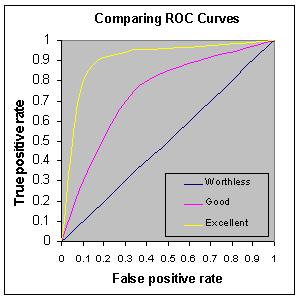
\includegraphics[width = (\textwidth)/2]{roccomp.jpg}
  \caption{Example of a ROC curve}
  \label{fig:ROC}
\end{figure}


With the research conducted in this section an approach of using several metrics seems to be the best choice to evaluate the research artefact. Some of these could be ROC curves and MAE. Specific metrics that will be used will be further researched and decided upon at a later date.\\ \\

%\cite{6608492}

\section{Conclusion}
In conclusion the literature explored in this chapter has helped to guide the development of the research artefact. Neural Networks was the algorithm chosen to train the model on. Data scraping was looked into further for collecting data to build a data set, but was not used more on this can be found in the data set chapter. Evaluation metrics used to aid in the evaluation of the model came from within the literature, confusion metrics were printed for each implementation of the model so a quick analysis could be done to compare the latest iteration to the previous. 
\chapter{Background Research}\label{ch:Background Research}
This chapter provides some background research on the conclusions of the literature review. Mainly looking into the algorithm a how training the model works. All things that were investigated during the implementation stage of the research artefact are discussed in this chapter.

\section{Algorithm}
The algorithm chosen from the papers in the literature review to be most relevant to use was the Neural Network algorithm. This algorithm can be used for both regression and classification tasks. In this instance a classification neural network algorithm is to be used. A neural network is a parallel, distributed information processing structure consisting of processing elements (units or nodes) interconnected together \cite{118638}. Examples of different neural network architectures can be seen in figure \ref{fig:NNA} below. Taken from \cite{485891} 
\begin{figure}[h!]
  \centering
  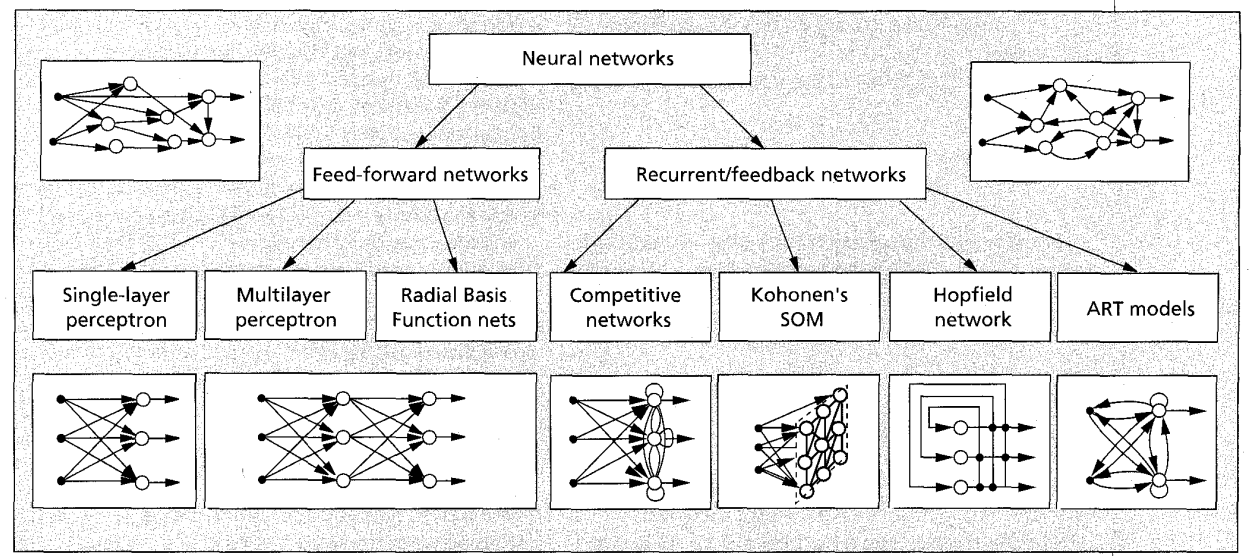
\includegraphics[width = (\textwidth)/2]{nnarc.png}
  \caption{Examples of different neural network architectures}
  \label{fig:NNA}
\end{figure}

A neural network works by passing in the data to the input layer which passes the data onto the hidden layer(s) ( the more complex a Neural Network, the more hidden layers it may have). On the hidden layer the neuron calculates the sum of the weights passed onto it. This then triggers an activation function which,the goal of an activation function is to define the output of a neuron's weighted input \cite{samatin_njikam_zhao_2016}. Once the prediction has been made the output is compared to the target input.The difference between the two patterns of output then determines how the weights are altered. Each particular recipe for change constitutes a learning rule \cite{Gurney1997AnIT}.

\section{Neural Network Learning Process}
The main learning process for a classification Neural Network (NN) involves a type of learning call supervised learning. In supervised leaning the training set includes the input patterns as well as the correct results. then after the output is given if the output is wrong the weights can be adjusted according to the difference \cite{kriesel}. A flowchart of supervised leaning can be seen below in figure \ref{fig:slfc}. Taken from \cite{seb}. 
\begin{figure}[h!]
  \centering
  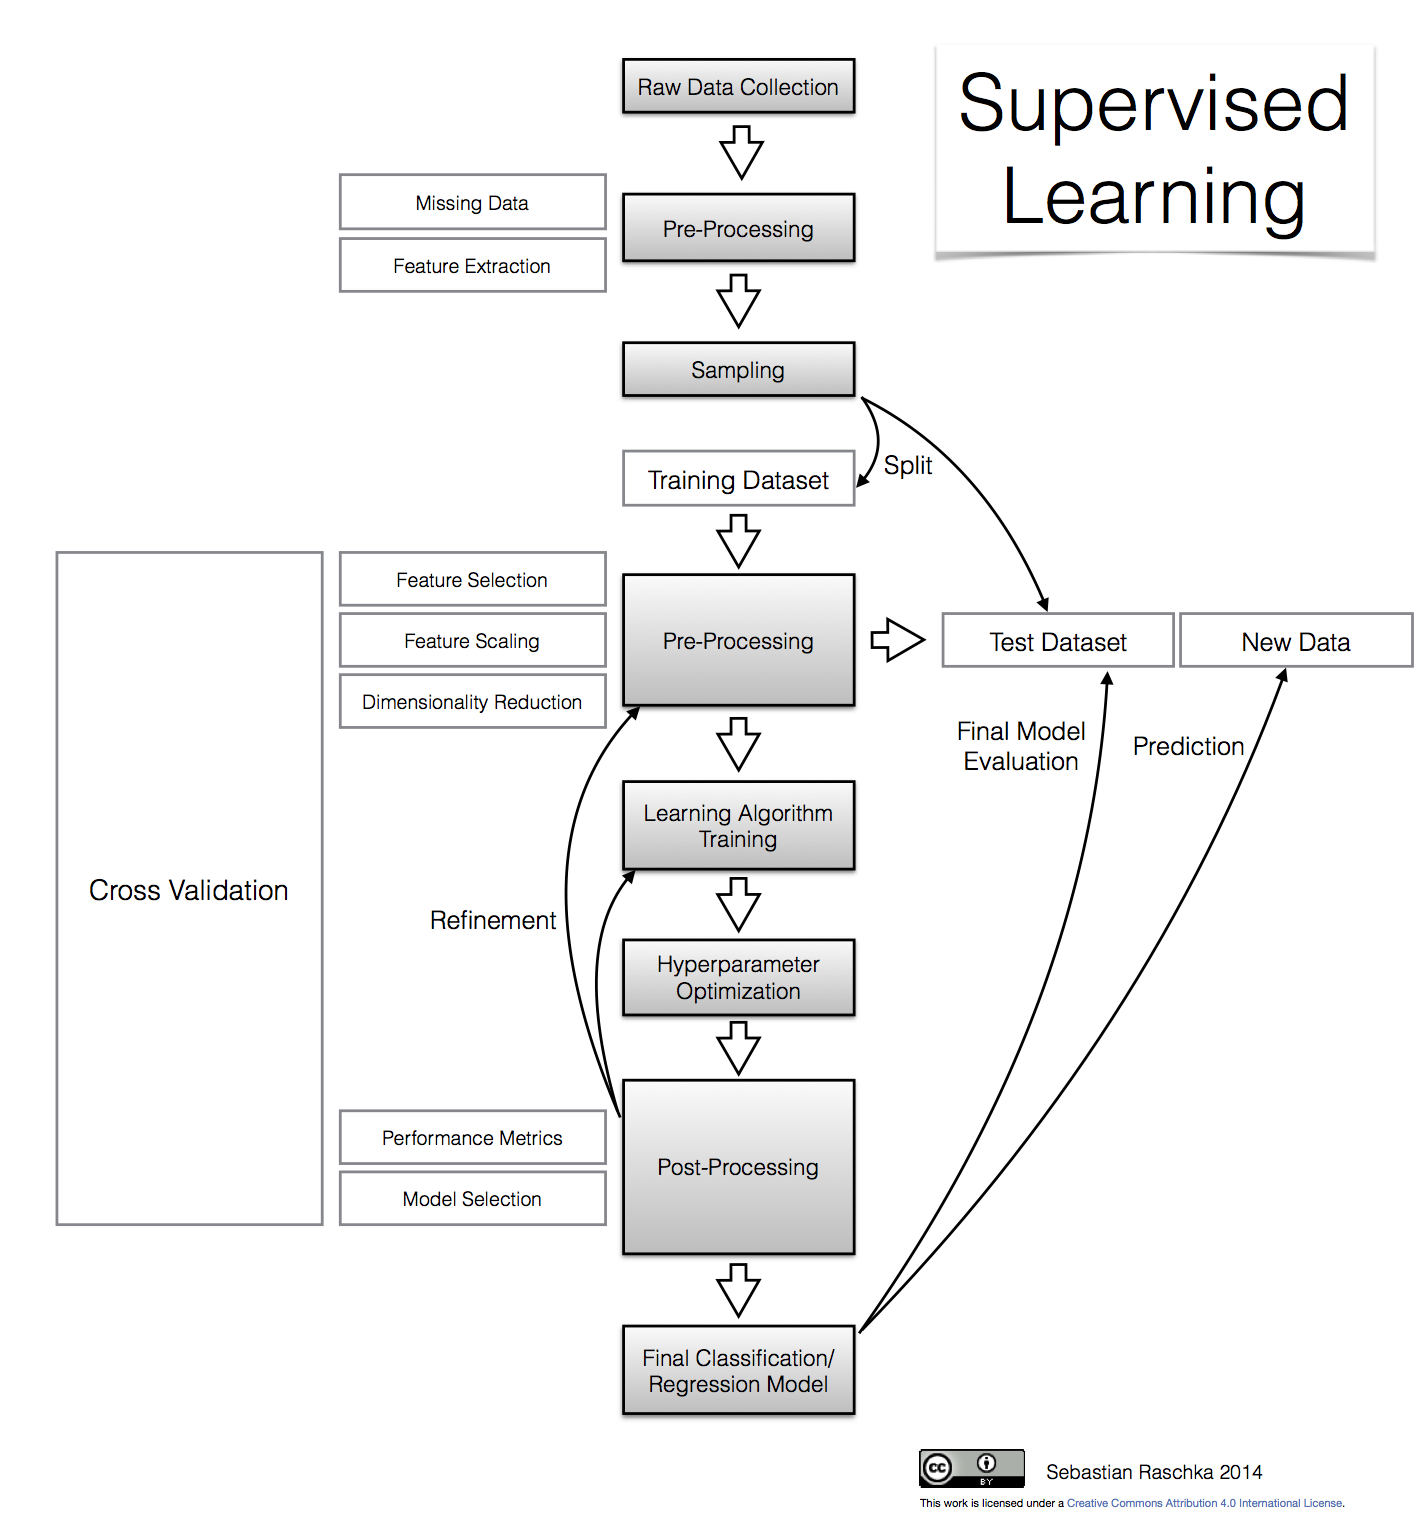
\includegraphics[width = (\textwidth)/2]{supervisedlearningflowchart.png}
  \caption{A flowchart showing the supervised learning process}
  \label{fig:slfc}
\end{figure}

\section{Conclusions}

With this extra background research and the conclusions of the literature review the design stages of the research artefact model can take place. Following on from this the research means that the knowledge needed for the implementation of the research artefact software can take place with ease. 





\chapter{Design}\label{ch:Design}

This chapter looks at how the research artefact was designed to complete the research for this project and meet the aims and objectives laid out before.

\section{Methodology of the Research Artefact}
The chosen method for the development of the system is the iterative approach (Figure \ref{fig:ITA}). This allows for continuous development of the system. As seen below after the planning and research has taken place the implementation of the system can begin. Once this has finished, testing takes place, if the system does not meet requirements during the testing stage a second iteration of the development can start, and more implementation can take place
\begin{figure}[h!]
  \centering
  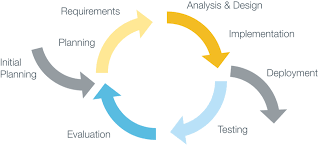
\includegraphics[width = (\textwidth)/2]{iterative.png}
  \caption{Diagram of the Iterative Approach}
  \label{fig:ITA}
\end{figure}\\

\section{Requirements of the Research Artefact}
\begin{itemize}
    \item The artefact needs to take an input of race data then produce an output of a predicted winner or non winner label based on the features of that horse.
    \item The artefact needs to correctly predict the winner to some acceptable degree of accuracy.
    \item The artefact could give and output of a probability of the horse winning as well as the predicted winner or non winner label 
    \item The artefact could allow for fresh race data so a prediction can be made on an upcoming race.
    
\end{itemize}

\section{Dataset Design}
During the literature review, data collection techniques were looked at as a way of building the data set. Whilst implementing a data scraper an observation of the data set built was that there wasn't enough data to train a model on, due to not being able to collect enough features to train the model off of. Because of this a decision was made to use a pre-existing data set. The data set is from \url{www.ukhorseracing.co.uk}. The data set before preprocessing has four hundred and seventy two features, and has 1,137,865 rows. The data contains over eighty thousand races from the past ten years for the model to be trained off of. Due to the size of the data set it was believed that a model could be trained to a higher accuracy then if the model had been trained off of a data set built from collected data via scraping.

\section{Model Design Approach}

The model will work in a similar way to the flowchart below ( Figure \ref{fig:FC}). As seen by the flowchart the research artefact software will view if the data needs preprocessing or not, then it will split the data, train the model, then predict the outcome. This is a very basic implementation as there is more sub processes that will take place and some may need to be implemented further on. An example of a sub process that was implemented further on was SMOTE, an oversampling technique to try and reduce over fitting in a machine learning model.
\begin{figure}[h!]
  \centering
  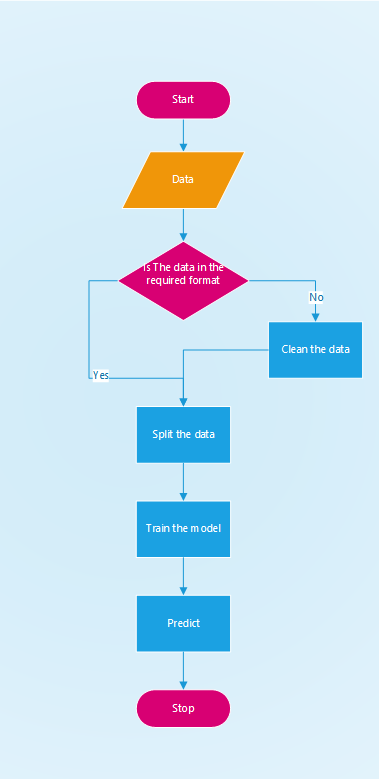
\includegraphics[width = (\textwidth)/2]{flowchart.png}
  \caption{Basic flowchart of model implementation}
  \label{fig:FC}
\end{figure}


\section{Conclusions}
In conclusion the aspects of design touched upon in this chapter have greatly aided the production of the research artefact software implementation. Without the designs discussed above the time taken to produce the research artefact software would have been considerably longer. 

\chapter{Dataset}\label{ch:Data}

This chapter examines the data set used in this project. It looks at how the data set is laid out to how the data was explored prior to preprocessing and training the model. 

\section{Dataset Origin}
The origin of the data set was previously discussed in the design chapter under the data set design section. The size of the data set is also mentioned in the chapter above.

\section{Data Exploration}
Learning the data set is an important stage to complete before training the model. It is useful as you can tell what the data set looks like to judge how much preprocessing takes place. some of the graphs and findings of the data exploration phase are examined below. The reason to explore data is to look for normality in the distributions of features, as well as looking for skewness and kurtosis.


The graph below shows a sample of the data set with the missing values being marked by a white cell and a valid sample as a black cell. the reason for it being only a sample of the data set is due to the size of the entire data set and the hardware available not being capable of running this missing data visualisation. This graph was produced using the missingno library.\\\\\\\\

\begin{figure}[h!]
  \centering
  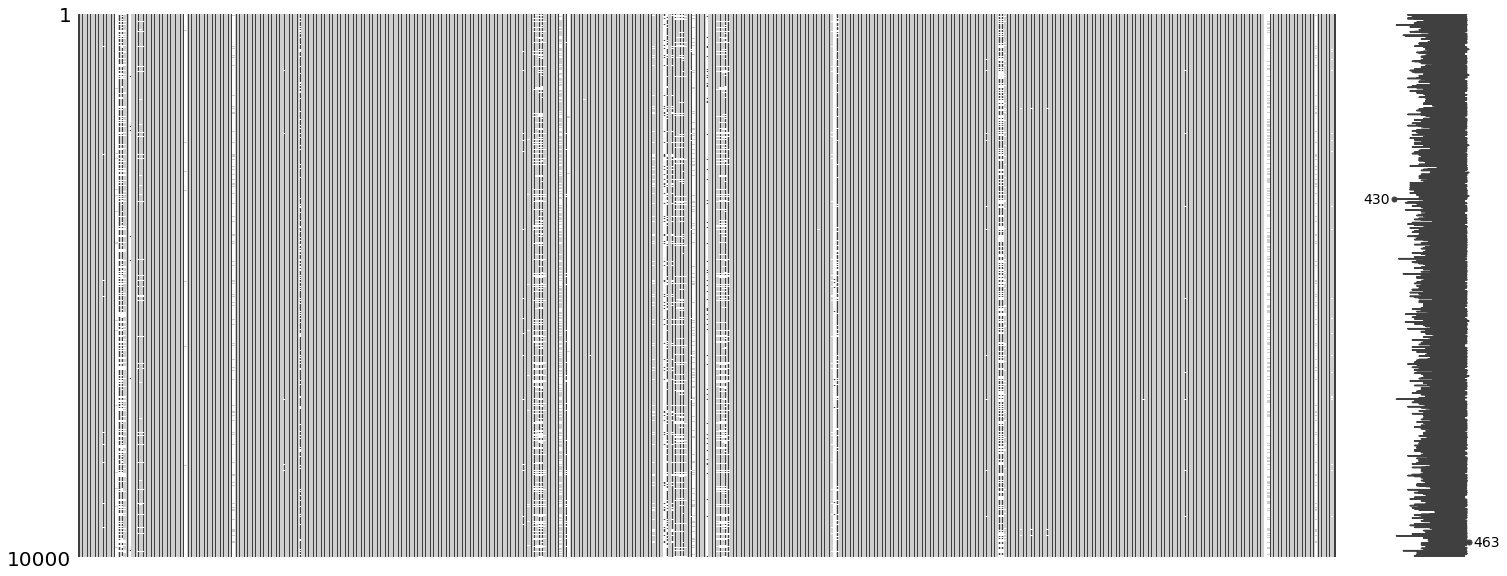
\includegraphics[width = (\textwidth)/2]{missingVals.png}
  \caption{Missingno matrix showing missing data for the first 10,000 samples}
  \label{fig:MV}
\end{figure}

As seen by the missing values matrix (figure \ref{fig:MV}) most of the features are either complete with only a few missing data or having non at all. The spark line on the side of the graph shows the completeness of the data on each row, with the maximum and the minimum marked out.Some of the features were then looked at to see the distribution of feature sets. The distribution for the furlongs of a race can be seen below.As you can see five furlongs seems to be the most common race length throughout the data set. 
\begin{figure}[h!]
  \centering
  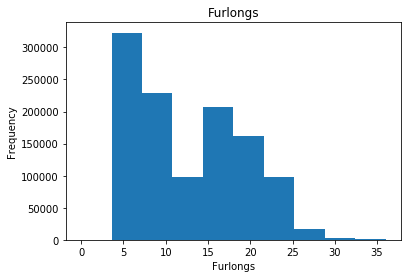
\includegraphics[width = (\textwidth)/2]{furlongs.png}
  \caption{furlongs distribution}
  \label{fig:fur}
\end{figure}

The horses age is another example of on of the features looked at below the distribution for the horses age for the whole data set can be seen along side a box blot showing the quartile ranges of the feature. As seen by figure \ref{fig:had} the most common age in the data set for horses is 4 years old, with the median being 5 as seen in figure \ref{fig:hab}. A further breakdown of the horses age by winner and non winner are discussed below.
\begin{figure}[H]
  \centering
  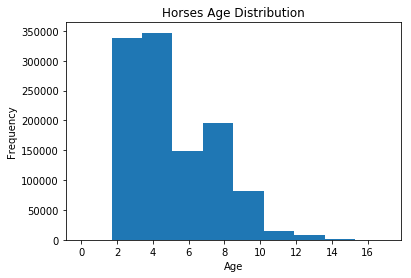
\includegraphics[width =(\textwidth)/2]{HorseAgeDistro.png}
  \caption{Horses age distribution}
  \label{fig:had}
\end{figure}
\begin{figure}[H]
  \centering
  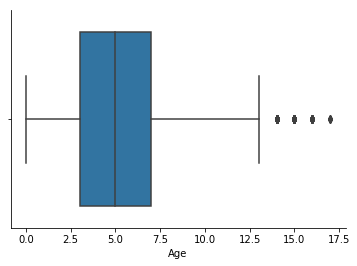
\includegraphics[width =(\textwidth)/2]{HorseAgeBoxplot.png}
  \caption{Horses age box plot}
  \label{fig:hab}
\end{figure}

As discussed further into this report, the model was changed to predict just a winner and non winner of the race. The visualisation of the distributions of the horses age for these labels can be seen below. As seen in figures \ref{fig:hawd} \& \ref{fig:hald} there is no underlying distribution to either category suggesting there is a level of randomness to the age of the winner horse, except for that most horses in this data set are 4 years old. 
\begin{figure}[H]
  \centering
  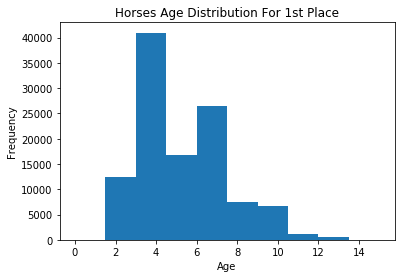
\includegraphics[width =(\textwidth)/2]{winnersAgeDistro.png}
  \caption{Horses age for 1st place distribution}
  \label{fig:hawd}
\end{figure}
\begin{figure}[H]
  \centering
  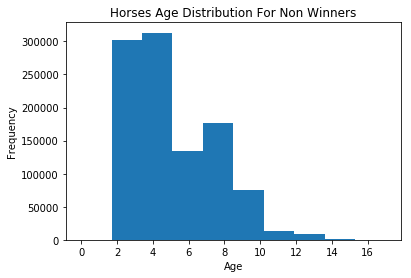
\includegraphics[width =(\textwidth)/2]{download.png}
  \caption{Horses age distribution for non winners}
  \label{fig:hald}
\end{figure}

\section{Conclusions}
The data within the data set is understood and the steps towards making the data set usable for training a neural network are clear and will take place during the preprocessing stage. Some of these steps will be talked about during the preprossessing section in the implementation chapter.


\chapter{Implementation}\label{ch:Implementation}

This chapter examines the implementation of the project in its main stages. Firstly, the way the data was preprocessed for the model will be discussed. Then the way the model was implemented and the iterations the model went through. 

\section{Development Tools}
This section will look at the hardware and software that was used for the production of the research artefact to achieve the aims and objectives.
\subsection{Hardware}
No specialist hardware was required for this project. Only a computer was needed on the hardware side of things.
\subsection{Software}  
The software that was required for this project was a development environment to program in, the chosen development environment for this project was Jupyter Notebook. In addition to the use of a IDE, certain libraries were used for both the preprocessing of the data set and for building the actual model. The libraries needed for this project to aid in the research are listed below with an explanation of why and how they were used.
\subsubsection{Data Preprocessing Libraries}
\begin{itemize}
    \item Pandas is a library to make handling a data set easy to do by using a custom data frame type to store the data. when the data set was first received it was broken up into the races from each month for the past ten years. To leverage the data easily, the data was merged into one larger data set. Pandas was used for this and then handling the data throughout the preprocessing stage up until it was split into training and testing for the model. 
    \item Missingno was used to look at a small sample of the data set to quickly visualize the completeness of features in the data set. 
    \item pyplot is a part of the matplotlib library and was used to create graphs during the data explorations phase.
    \item seaborn was also used to create graphs, especially box plots to look at the quartile ranges of feature sets. 
    \item Label encoder  from sklearn preprocessing was used to encode the string labels to numbers so they can then be normalized for the input to the neural network.
    \item normalize was used to normalise the x values for the algorithm.
\end{itemize}
\subsubsection{Model Building Libraries}
\begin{itemize}
    \item SMOTE from imblearn oversampling was used to minimise an over fitting issue that was encountered 
    \item train test split sklearn model selection was used to split the ddata up into the training and the testing subsets.
    \item MLP classifier from sklearn neural network was the algorithm used for the neural network classification task. 
\end{itemize}
\subsubsection{Evaluation and Testing Libraries}
The below were all used to gather metrics that could be used to evaluate the model.
\begin{itemize}
    \item classification report from sklearn metrics.
    \item confusion matrix from from sklearn metrics.
    \item accuracy score from sklearn metrics.
\end{itemize}

\section{Data Preprocessing}
This section will talk through the steps taken to get the data set ready for training the leveraged algorithm to produce the research artefact.

\subsection{Loading the Dataset}
Loading the data set was done using the pandas library, the data set was loaded into a data frame to make it easy to manipulate. 

\subsection{Handling Missing Data}
The way in which missing data was handled depends on the feature, some features were deleted if that column in the data set was completely and some had values placed into the n/a that appeared in the data frame once it had been imported. Some examples of the data imputated and the reasoning for the imputated values will be mentioned now, as well as the reasoning for deleting some of the features. Some examples of the imputated data are: The feature 'actual going' had unknown as a label in the data set. Twelve thousand samples were missing due to this and unknown already being a part of the feature the value unknown was imputated for the missing values. Another value that was imutated was country was set to UK if it was unknown as all raced happened within the UK. Some of the empty values that were deleted as the were deemed to not affect the model if they had been filled in are the ones where information had to be written in or the odds of the race in a different format that had to be worked out. 

\section{Building the Model}
This section will walk through how the model was built and improved upon through several iterations. Mentioning how the models were improved and how they differ from the previous iteration. All the iterations follow the methodology previously stated that this project will follow. 

\subsection{Iteration One}
Once the data set had been preprocessed building a model could begin. The first step was too split the data into the x and y for the model, all features apart from result were the x and result was y. Result was the y variable as this was what we were trying to predict. The train test split was seventy, thirty respectively for the first iteration. The next stage was to encode all the features that were not already numbers. This was needed as you cant noramlise a non number type. the next stage of buliding the model was to noralise the input data for the neural network. this stage is important due to variables needing the same range of variance because the underlying probability density function is to be estimated with a kernel of the same width in each dimension \cite{97934}. The last stage of building the model is to fit the training data to the algorithm. The model at this stage had not been optimised and has had no parameter tuning.The results of the first iteration of this implementation are discussed below: 

Due to the feature of result having so many labels to predict in this model such as the place from first up to thirty-third in one case due to the size of that race case, as well as  labels such as being disqualified, falling, and unseating the rider as a possible race finish for a said horse, the accuracy was quite low. The accuracy as a preliminary result for the model was 0.28 or 28\%. the confusion matrix for this model can be seen below (Figure \ref{fig:M1CF}).
\begin{figure}[h!]
  \centering
  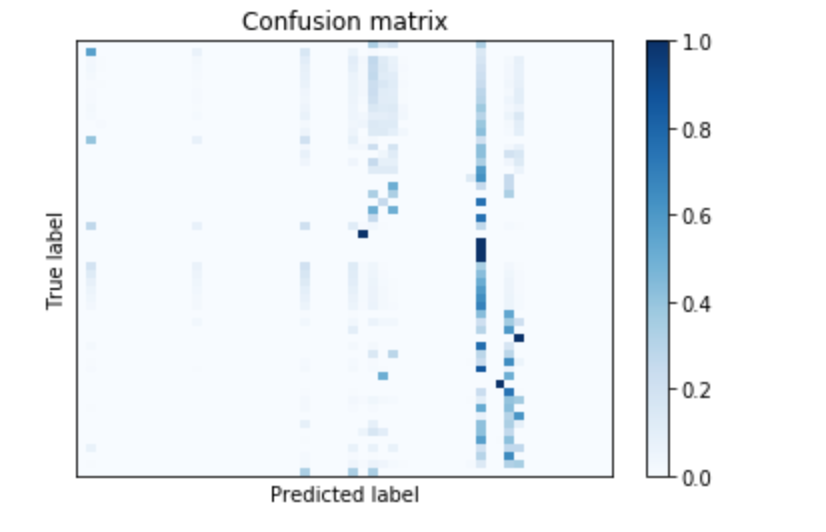
\includegraphics[width = (\textwidth)/2]{model1.png}
  \caption{Model one confusion matrix}
  \label{fig:M1CF}
\end{figure}
\subsubsection{Iteration One Conclusion}
From looking at the confusion matrix you can see the model struggles to predict the majority of the labels, which causes the model to have a low accuracy score. The improvements made in the next model is a change to the labels of the predicted feature. The results of this change is discussed below in the iteration two section. 


\subsection{Iteration Two}
As previously discussed the improvements made for the second iteration was a change to the labels it was predicting. The change that was made was the label for first place stayed the same and all other labels were changed to 0, the reasoning behind this is that for the purpose of the model any position other than first was a non winner or a loser of the race.

The way in which the label was changed was looking at any label that was not currently 1 and changing the label to 0. All other stages of building the model were the same. The data was split the same way across the same ration of training and testing. Then encoded, normalised and finally fitted to the models algorithm. The results for this iteration are as follows. The model had a greatly improved accuracy with with an accuracy score of 0.90 or 90\%. This high accuracy was caused by an over fitting of the model to the losing label. 
\begin{figure}[h!]
  \centering
  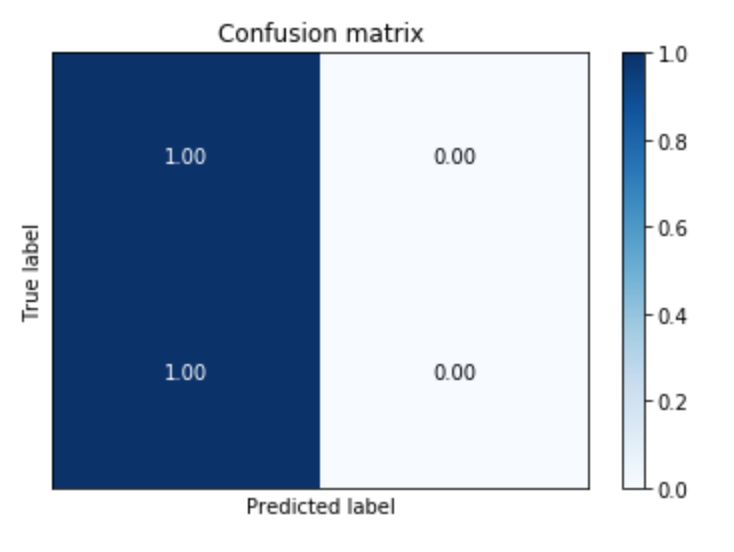
\includegraphics[width = (\textwidth)/2]{model2.png}
  \caption{Model two confusion matrix}
  \label{fig:M2CF}
\end{figure}

\subsubsection{Iteration Two Conclusion}
As you can see by the confusion matrix for this Iteration (Figure \ref{fig:M2CF}) the model was only predicting the losing label and not trying to predict the winning label at all. This is due to there being more losers to a race than a single winner so the model over fitted to that label in the predicted feature. A solution to over fitting data is implemented in the third iteration of the model. 

\subsection{Iteration Three}
The third iteration of the models implementation looks at implementing a solution to the over fitting to the loser label. The solution explored and implemented was using SMOTE. Synthetic Minority Over-sampling Technique. The way SMOTE works is by generating synthetic examples for the minority class by taking the minority class sample and introducing the synthetic one by joining any of the line segments of the k minority class neighbour \cite{SMOTE}.

This model was built slightly differently to the other two as it has SMOTE implemented. All the preprocessing of the data set is the same. The train test split is different on this model as it is moving closer to being trained on the whole data set. This time its split ninety, ten, for training and testing respectively. Then After encoding the values the same way as before, SMOTE is applied to the training data only. The reason for only over sampling the training data is so none of the testing data is used to create synthetic observations, to try and keep the results generalisable.

In using this technique to try to reduce over fitting of the loser data, some success was had. The accuracy score did drop to 0.77 or 77\%. But the precision and recall of the winner label went from 0,0 to 0.24,0.61 respectively, an improvement on before.
\begin{figure}[h!]
  \centering
  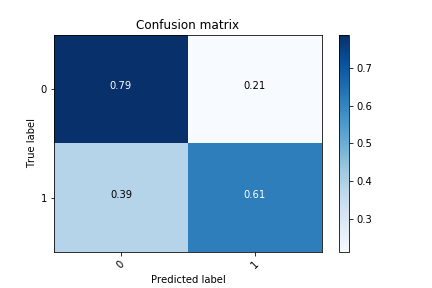
\includegraphics[width = (\textwidth)/2]{confusionMatrix.png}
  \caption{Model three confusion matrix}
  \label{fig:M3CF}
\end{figure}
\subsubsection{Iteration Three Conclusion}
As seen in the confusion matrix for the third iteration (Figure \ref{fig:M3CF}) a massive improvement on the accuracy of both predicting all labels from model one and predicting the winner from model two has been met with the implementation of changing the labels and an over-sampling technique to reduce over fitting has been achieved. But further steps need to be taken in the next iteration of the model a cross validation technique will be implemented to try and further reduce the over fitting.
\subsection{Iteration Four}
As stated previously a cross-validation technique was going to be implemented into this iteration to try and reduce the over fitting problem faced in the second iteration further. The cross validation technique used implemented in this iteration of the model is the k-fold cross validation technique. The model followed a similar implementation as the previous iterations. The data was preprocessed then a split for training data and a validation set took place on a ninety percent to ten split respectively. Then the sting labels were encoded to numbers, to then be normalised. Then SMOTE was applied to the training data to over sample the minority class of the winner label. The x values were then normalised so the neural network can accept them as the input, due to a neural network needing normalised inputs as discussed previously. The training data was then passed through the k-fold cross validation.

After the ten folds had completed the model was questioned to make a prediction. The results of the model are that it improved the accuracy score to 0.86 or 86\%, but the precision and recall of the winner label changed to 0.33, 0.42 respectively. Precision is loosely speaking how useful the results are whilst recall is how complete the results are. The confusion matrix for the model with k-fold cross validation can be seen below. 
\begin{figure}[h!]
  \centering
  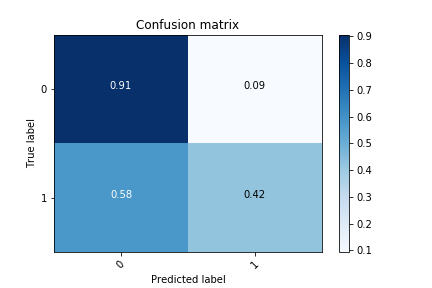
\includegraphics[width = (\textwidth)/2]{confusionMatrixkfold.png}
  \caption{Model four confusion matrix}
  \label{fig:M4CF}
\end{figure}
\subsubsection{Iteration Four Conclusions}
Implementing a cross validation technique led to an improved accuracy of the model, but the true positive score for the winning label was less than the previous iterations. This could be fixed with model optimization. the benefit of using cross validation is to reduce the chance of over fitting the model to certain classes in the data.  
\section{Conclusions}
 As seen throughout this chapter prediction models have been successfully implemented to predict the outcome of a horse race. A high level of accuracy in the later implementations has been achieved. An evaluation on the models built and the testing of the latest iteration will be discussed in the next chapter.
\chapter{Evaluation \& Testing}\label{ch:Evaluation}

This chapter evaluates the overall project and provides results of tests carried out upon the most recent iteration of the research artefact software. The evaluation part of this chapter examines the solution provided in the form of the research artefact, as well as, the research itself and what conclusions can be drawn from it. Testing interrogates the research artefact to see if it actually works. The difference between the testing and the evaluation is testing will see if the model works and the evaluation will look at how accurate the model is.  

\section{Evaluation}
As seen throughout the implementation chapter a predictive model for horse racing was successfully implemented to predict the outcome of the race, in the case of winner and non winners. This section will evaluate each of the models produced throughout the implementation process in further detail then the conclusions of each iteration.

\subsubsection{Iteration One}
As previously discussed model one did not have a result that could be classed as statistically significant. Although the accuracy was not very high the model could be classed as successfully implemented.
\subsubsection{Iteration Two}
After changing the predicted labels on for this model the accuracy did improve which was the goal. But the model had a major issue with over fitting. This model was expected to have that issue due to the difference in the number of samples for the two labels (see figures \ref{fig:hawd} \& \ref{fig:hald} for the difference in the number of samples). This was however improved upon in model three.
\subsubsection{Iteration Three}
Model three reduced the issue of over fitting that model two was experiencing due to a successful implementation of SMOTE to over sample the minority class in the prediction labels. Even with the drop in the accuracy this model can definitely be classed as an improvement on the previous models.  
\subsubsection{Iteration Four}
The final model of the implementation of the research artefact improved upon the previous model by adding in another measure to try and reduce over fitting. K-fold cross validation was the technique implemented to improve the model. The accuracy did improve upon the previous model, but the accuracy for the prediction of the winner label did was worse than the previous model. But because a cross validation technique was used during the training aspect of building this model the possibility of the model being either over fitted or under fitted to the data is reduced meaning that even though the accuracy is not as good as the previous model iteration, the prediction is more likely to be an accurate one compared to the previous iteration. 


\section{Testing}
This section will provide the results of the testing of the final iteration of the implemented research artefact software. Unit testing will be used to test the research artefact software. Unit testing is used to test all the individual functions of the research artefact software. To see the tests and the results of the unit testing see Appendix \ref{ch:appendixA}, Table \ref{tab:sidewaysTable}.
\section{Conclusions}
The evaluation stage only mentioned some of the basic analysis of the models, further analysis of comparisons of the label true positives and false negatives for each iteration of the research artefact implementations could take place, as well as a further in depth look at visualising the results for a better comparison and analysis.Other evaluation techniques could be used on the final iteration of the model, these include the Mean Absolute Error and the  Root Mean Square Error to help evaluate the final iteration further.
\chapter{Conclusion}\label{ch:Conclusion}

This chapter will summaries this projects outcomes and conclude on the conclude of the results from this body of work. The future work section will also highlight and further improvements or research that could take place with more time and resources. 


\section{Conclusions}
This section will see if the project objectives have been met and what chapter they were met. From the literature review it was apparent that knowledge of research into this filed would be pinnacle to producing the research artefact software. And meeting all objectives may be a difficult task, but as seen below the objectives for this project were all successfully achieved.
\begin{enumerate}
    \item Objective one and two was met during the literature review. See chapter \ref{ch:Literature Review} for the literature review where these objectives were met
    \item The third objective was met during the literature review during chapter \ref{ch:Literature Review}. But the method found was not used as the data set was collected from a website (see chapter \ref{ch:Data}) instead of being scraped from the internet.
    \item Objective 4 was met during the implementation stage (chapter \ref{ch:Implementation}). It was successfully met as there were many models implemented that predicted the outcome of a sporting event, in particular a horse race.
    \item After evaluation techniques were collected in chapter \ref{ch:Literature Review}, they were used to evaluate in chapter \ref{ch:Evaluation}. Meaning objective five has been achieved. 
\end{enumerate}

\section{Future Work}
Some of the further research and improvements are within this section. The model could be improved by allowing an input of raw data that has never been seen before, preprocessing it, then running a prediction against the trained model to then predict the winner of that race. This could be a future race that has not happened yet. As well as predicting the horse as a winner the system could give a probability of that horse winning. Further research could be done into the hyper parameters the model could have to help optimize and improve the model. 

 %NOTE: reduced the size of the text for the bibliography
%NOTE: set the style for the bibliography and display the references used within the document

%  http://tex.stackexchange.com/questions/67153/bibliography-not-in-toc-when-using-biblatex-biber
%\printbibliography[heading=bibintoc]
\footnotesize
\nocite{*}
\addcontentsline{toc}{chapter}{Bibliography}
\bibliography{thesis}
\normalsize
\appendix
\chapter{Unit Test Table}\label{ch:appendixA}
\begin{sidewaystable}[h!]
\begin{center}
       \begin{tabular}{|p{1cm}||p{3cm}|p{10cm}|p{5cm}|p{3cm}|p{2cm}| }
   \toprule
   \textbf{Test} & \textbf{Name}  & \textbf{Description}  & \textbf{Expected Outcome}  & \textbf{Actual Outcome}  & \textbf{Result} \cr
   \midrule
   1 &  open data set  & test that the pandas read csv opens the data set correctly and returns it as the correct type & The data set is opened and a data frame is returned & as expected & pass  \cr
   2 &  label encoder & test that all labels are encoded and no stings are left & no strings are left all labels are encoded & as expected & pass  \cr
   3 & data split & see if train test split correctly splits the data set & the training set has 90 \% of the data in  & as expected & pass  \cr
   4 & Normalise & Normalising the data is correctly executed & all data is normalised & as expected & pass  \cr
   5 & training the model  & the model is trained and no errors occur during this phase  & a trained model & as expected  & pass  \cr
   6 & test the prediction & the model give a valid prediction after being given values that should give a 100\% accuracy & the prediction is 100\% accurate & as expected & pass
   \bottomrule
   \end{tabular}
\caption[Unit testing table]{
	A table showing the unit tests and test results.}
\label{tab:sidewaysTable}
\end{center}
\end{sidewaystable}

%\includepdf[pages={1}]{scan.pdf}


\begin{figure}[h!]
\includegraphics[scale=0.75]{scan.pdf}
\end{figure}
\end{document} %NOTE: END of document, nothing after this point
